%%
%% Customizações do abnTeX2 (http://abnTeX2.googlecode.com) para a Universidade XXXX
%%
%% This work may be distributed and/or modified under the
%% conditions of the LaTeX Project Public License, either version 1.3
%% of this license or (at your option) any later version.
%% The latest version of this license is in
%%   http://www.latex-project.org/lppl.txt
%% and version 1.3 or later is part of all distributions of LaTeX
%% version 2005/12/01 or later.
%%
%% This work has the LPPL maintenance status `maintained'.
%% 
%% The Current Maintainer of this work is SEU_NOME, SEU_EMAIL
%%
%% Further information about abnTeX2 are available on https://github.com/abntex/abntex2
%%

% ---
% INICIO DAS CUSTOMIZACOES PARA A FACULDADE UNB GAMA
% ---

\newcommand{\curso}[1]{\def\imprimircurso{#1}}

\newcommand{\palavraChaveUm}[1]{\def\imprimirpalavrachaveum{#1}}
\newcommand{\palavraChaveDois}[1]{\def\imprimirpalavrachavedois{#1}}

\newcommand{\cdu}[1]{\def\nomecdu{#1}}
\newcommand{\dataDaAprovacao}[1]{\def\imprimirdatadaaprovacao{#1}}

\newcommand{\membroConvidadoUm}[1]{\def\imprimirmembroconvidadoum{#1}}
\newcommand{\membroConvidadoDois}[1]{\def\imprimirmembroconvidadodois{#1}}

\newcommand\BackgroundPic{%
	\put(0,0){%
		\parbox[b][\paperheight]{\paperwidth}{%
			\vfill
			\centering
			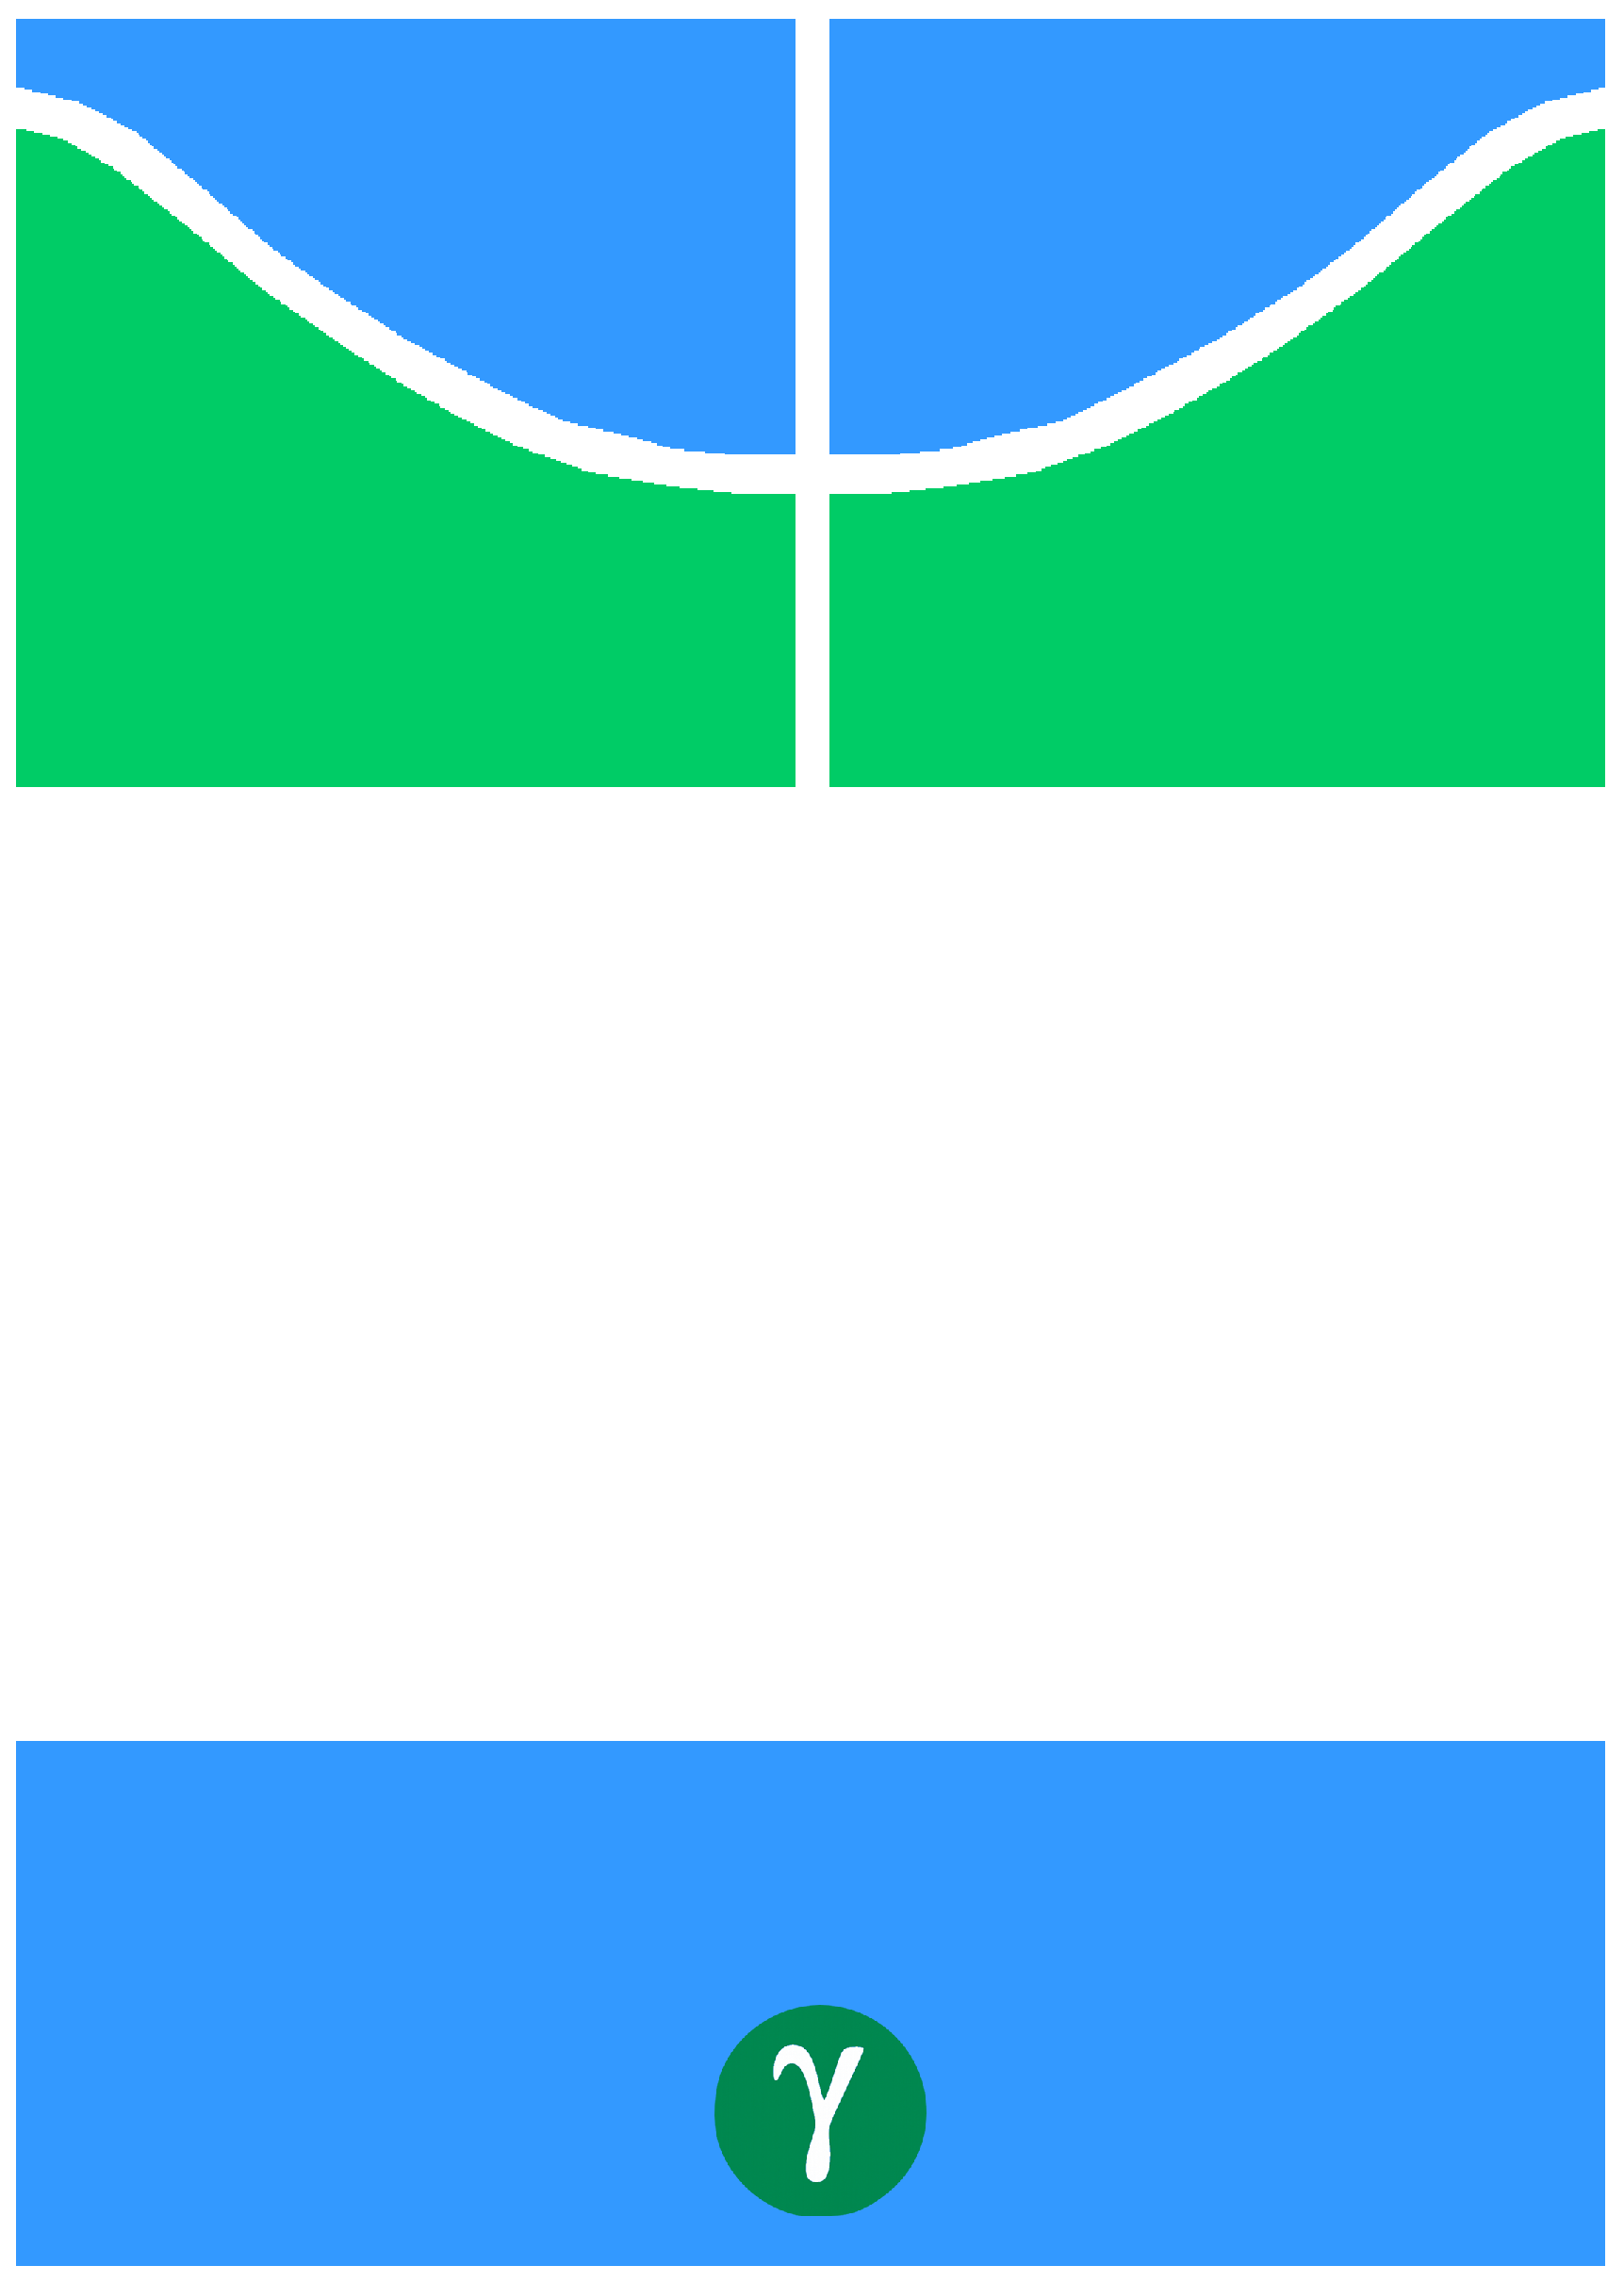
\includegraphics[width=\paperwidth,height=\paperheight,%
				keepaspectratio]{figuras/capa.eps}%
			\vfill
		}
	}
}

\renewcommand{\imprimircapa}{%
  \begin{capa}%
    \center
	\AddToShipoutPicture*{\BackgroundPic}

%	\begin{huge}
%		\textbf{\textsc{Trabalho de Conclusão de Curso}}
%	\end{huge}

    \vspace*{2.9in}
	{\textbf{\large\imprimirinstituicao}}
	\par
	{\textbf{\large\imprimircurso}}

	\vspace{1.5in}

    {\ABNTEXchapterfont\bfseries\LARGE\imprimirtitulo}
    \vspace*{\fill}
    
	\begin{flushright}
    	\textbf{{\large{Autor: \imprimirautor}}}
		\par
    	\textbf{{\large{Orientador: \imprimirorientador}}}
	\end{flushright}
		
    \vspace*{0.2in}
    \textbf{{\large\imprimirlocal}}
    \par
    \textbf{{\large\imprimirdata}}
    
    \vspace*{1in}
  \end{capa}
}

% ---
% FIM DAS CUSTOMIZACOES PARA A FACULDADE UNB GAMA
% ---


